\documentclass{book}

\usepackage[utf8]{inputenc}
\usepackage[T1]{fontenc}
\usepackage[francais]{babel}
\usepackage{graphicx}
\usepackage{adjustbox}
\usepackage{fancyref}
\usepackage{hyperref}
\usepackage{url}
\usepackage{amsmath} % pour les cascades de fraction
\usepackage{colortbl} % bfseries pour mettre une colonne en gras
\usepackage[top=1cm, bottom=1cm, left=1cm, right=1cm]{geometry} % pour les marges


\title{%
  Projet de Sciences des Données \\
  \large Explotation d'images satellites haute-résolution \\pour la prévision d'indicateurs socio-économiques \\
    }

\author{\textsc{Youcef} - \textsc{Kacer}}
\date{22 Novembre 2016}

\begin{document}
 
\maketitle

\tableofcontents

\frontmatter
\chapter{Introduction}
Dans ce document, nous présentons les premiers résultats de régression et de classification des communes françaises, à partir de leur histogramme de $NDVI$. 
Nous cherchons ainsi à prédire la densité de population de chaque commune.\\
Nous verrons comment ont été selectionnées les scènes \begin{itshape}Landsat-8\end{itshape} pour le territoire français à partir desquelles on extrait le $NDVI$ de chaque commune.\\
Ensuite, nous présenterons d'abord le problème d'apprentissage comme un problème de régression où on cherche à prédire la densité comme valeur continue, à partir
des histogrammes de $NDVI$ des communes. Puis, nous simplifierons le problème en catégorisant la densité, nous ramenant ainsi à un problème de classification.\\
Les techniques d'apprentissage utilisées seront très variées et on s'attachera à les comparer entre elles via un critère de performance.

\mainmatter
\chapter{Données Landsat-8 pour la France métropolitaine}

Une scène \begin{itshape}Landsat-8\end{itshape} correspond à une certaine zone de la Terre couverte périodiquement (16 jours) par le satellite. 
Elle est identifiée par un \begin{itshape}path\end{itshape} (typiquement entre
$192$ et $204$ pour la France) et un \begin{itshape}row\end{itshape} (typiquement entre $023$ et $032$ pour la France).\\ 
Nous avons récupéré des scènes Landsat-8 couvrant la France métropolitaine entre le 15 Mai 2013 et le 15 Septembre 2013.\\
La figure \ref{selection_france} montre le polygone de sélection des scènes sur l'interface du site de l'$USGS$ \cite{landsat8}.

\begin{figure}[H]
\begin{center}
\includegraphics[scale=0.5]{images/france-selection.png}
\end{center}
\caption{Polygone de sélection des scènes $Landsat-8$ pour la France sur l'interface du site de l'$USGS$}
\label{selection_france}
\end{figure}

\clearpage

Cette période correspond à l'année des valeurs de densité de population à notre disposition pour l'ensemble des communes de France.\\
La période de Mai à Septembre est la plus courte permettant de couvrir tout le territoire métroplitain tout en conservant une occupation
nuageuse inférieure à 20\%.
Nous obtenons ainsi 70 scènes Landsat-8 chacune correspondant à un couple $path$,$row$ unique.\\
Les figures \ref{cloud1},\ref{cloud3},\ref{cloud4} et \ref{cloud5} montrent des miniatures couleurs des 4 scènes parmi les 70, ayant une couverture 
nuageuse supérieure à 10\%

\begin{figure}[H]
\begin{center}
\includegraphics[scale=0.2]{images/LC82000242013271LGN00.jpg}
\end{center}
\caption{Miniature couleur en projection Web Mercator (EPSG:$3857$) de la zone $200$,$024$ (region Nord-Pas-de-Calais) - couverture nuageuse de 20.00\% }
\label{cloud1}
\end{figure}


\begin{figure}[H]
\begin{center}
\includegraphics[scale=0.2]{images/LC82030252013196LGN00.jpg}
\end{center}
\caption{Miniature couleur en projection Web Mercator (EPSG:$3857$) de la zone $203$,$025$ (région des îles anglo-normandes) - couverture nuageuse de 18.30\%}
\label{cloud3}
\end{figure}

\begin{figure}[H]
\begin{center}
\includegraphics[scale=0.2]{images/LC81950262013156LGN00.jpg}
\end{center}
% \caption{Miniature couleur en projection Web Mercator (EPSG:$3857$) de la zone $195$,$026$ (poînte strasbourgeoise) - couverture nuageuse de 13.00\%}
\label{cloud4}
\end{figure}

\begin{figure}[H]
\begin{center}
\includegraphics[scale=0.2]{images/LC81950282013204LGN00.jpg}
\end{center}
\caption{Miniature couleur en projection Web Mercator (EPSG:$3857$) de la zone $203$,$028$ (frontière franco-italo-suisse) - couverture nuageuse de 12.60\%}
\label{cloud5}
\end{figure}

On voit donc que les scènes ayant une forte couverture nuageuse sont :
\begin{description}
\item[-] soit des scènes contenant beaucoup de domaine maritime
\item[-] soit des scènes limitrophes de pays voisins. 
\end{description}
La présence de nuage devrait donc avoir une faible impacte sur le $NDVI$ des communes françaises.
\clearpage

la figure \ref{couverture} présente toutes les scènes après projection en Web Mercator (EPSG:3857) (repère absolu).

\begin{figure}[H]
\begin{center}
\includegraphics[scale=0.7]{images/france-covering.png}
\end{center}
\caption{Concaténation des 70 scènes Lansat-8 après projection en Web Mercator (EPSG:3857)}
\label{couverture}
\end{figure}
\clearpage

\chapter{Extraction de l'histogramme de NDVI}

Nous avons à notre disposition un fichier de $36700$ comunes françaises contenant entre autres caractéristiques, les latitude et longitude en degrés,
la surface em km\textsuperscript{2}, la densité de population tel que recensée par l'INSEE en 2013 \cite{insee_pop2013}.\\
Afin d'obtenir des longitudes et latitudes précises, nous les avons corrigés en utilisant une API $Python$ de géolocalisation: $geopy$ \cite{geopy}.\\

La méthode d'extraction d'information du NDVI pour chaque commune se fait comme suit :
\begin{description}
\item[-] Pour une commune donnée, on projete ses latitude et longitude en Web Mercator. Les positions $x$,$y$ obtenues permettent d'aller récupérer 
la scéne \begin{itshape}Landsat-8\end{itshape} dont le centre est le plus proche de la commune. Prendre la scène la plus proche de cette manière,
permet d'éviter que la commune échoue sur un bord non couvert par une scène.
\item[-] Puis, on découpe un carré de centre les coordonnées de la  commune, et d'aire égale à la surface de la commune.
\item[-] On crée alors l'image de \begin{itshape}NDVI\end{itshape} correspondante
\item[-] On calcule l'histogramme de l'image de \begin{itshape}NDVI\end{itshape} en prenant 512 bins uniformément répartis dans l'intervalle [-1 1].
\item[-] On obtient ainsi un vecteur descripteur pour la commune
\item[-] On réitère le procédé pour chacune des communes
\end{description}


Nous présentons le procédé à travers l'exemple ci-après \ref{ndvi_extraction} :
\begin{figure}[H]
\centerline{
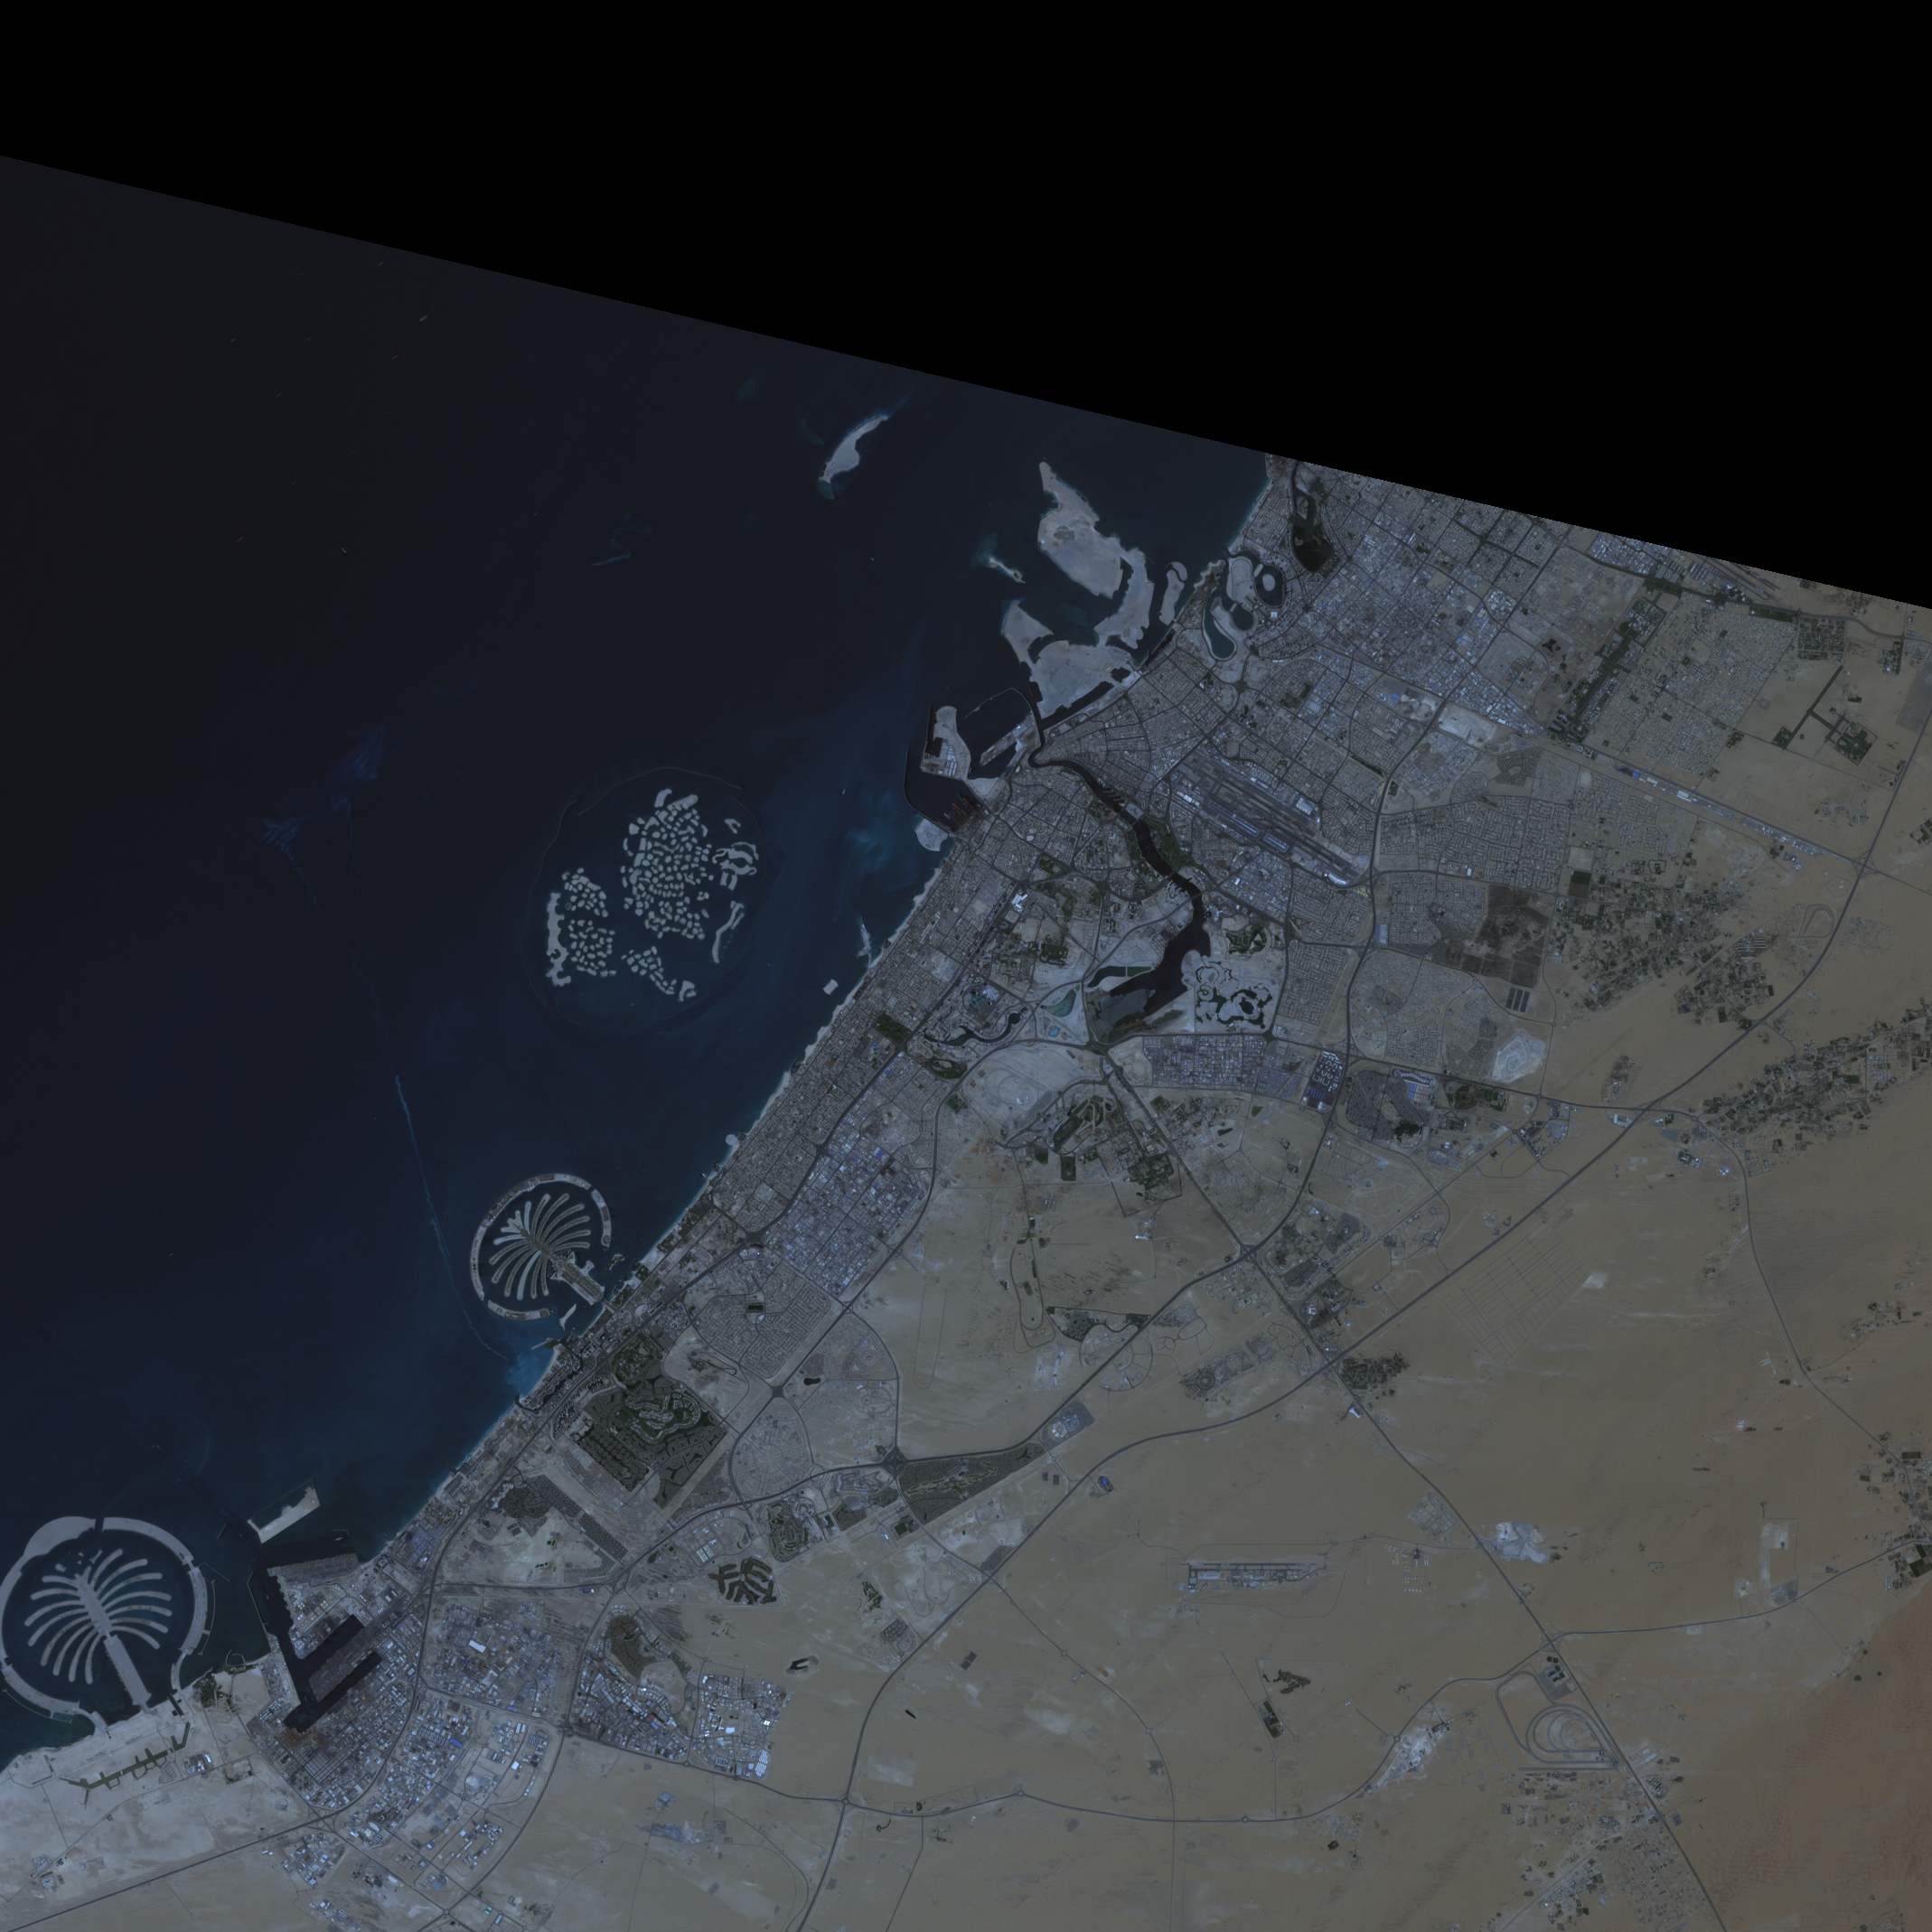
\includegraphics[scale=0.45]{images/05_rgb.png}
\includegraphics[scale=0.45]{images/05_ndvi.png}
\includegraphics[scale=0.4]{images/colormap.png}
}
\begin{center}
\includegraphics[scale=0.45]{images/05_ndvi_histo.png}
\end{center}
\caption{Image couleur, image $NDVI$ et histogramme de $NDVI$ pour la commune de $Carcassonne$ sur un périmètre de $65.08$km\textsuperscript{2} au mois de $Mai$ 2013}
\label{ndvi_extraction}
\end{figure}

\clearpage

Au final, nos données se présente sous la forme d'un tableau contenant à chaque ligne, l'histogramme d'une commune et sa densité. Avec un total
de $36139$ communes métropolitaines.\ref{data_reg}.

\begin{table}[H]
\begin{center}
\begin{adjustbox}{max width=\textwidth}
\begin{tabular}{|c|c|c|c|c|c|c|c|c|>{\bfseries}c|}

\hline 
nom &  bin-1 & bin-2 & ... & bin-255 & bin-256 &... & bin-511 & bin-512 & densité (habs/km\textsuperscript{2}) \\
\hline 
Ozan & 0 & 0 & ... & 1 & 5 & ... & 0 & 0 & 93.0\\
\hline 
Cormoranche-sur-saone & 0 & 0 & ... & 1 & 4 & ... & 0 & 0 & 107.0\\
\hline 
Paris & 0 & 0 & ... & 1953 & 1815 & ... & 0 & 0 & 21288.0\\
\hline
Lyon & 0 & 0 & ... & 1099 & 1032 & ... & 0 & 0 & 460.0\\
\hline
Tours & 0 & 0 & ... & 268 & 238 & ... & 0 & 0 & 3888.0\\
\hline
Besancon & 0 & 0 & ... & 97 & 122 & ... & 0 & 0 & 1797.0\\
\hline 
... & ... & ... & ... & ... & ... & ... & ... & ... & ... \\
\hline
\end{tabular}
\end{adjustbox}
\end{center}
\caption{Variables explicatives (histogramme de $NDVI$) et variable à prédire (densité) par régression, sous forme de tableau}
\label{data_reg}
\end{table}

\clearpage

Nous avons donc à présent des données sous forme de tableau prêt à être utiliser pour l'apprentissage supervisée.

\chapter{Régression pour la prédiction de densité de population en fonction du NDVI}

\section{Erreur de généralisation d'un modèle de régression}

Nous avons testé plusieurs algorithmes (ou modèles) de régression, du plus simple (régression linéaire) au plus élaboré (forêt aléatoire d'arbres régressifs).
Chacun de ces algorithmes est évalué par cross-validation. \\
C'est-à-dire qu'on compose plusieurs sets à partir des échantillons de départ. Chaque set contient un sous ensemble
aléatoire des échantillons pour l'entraînement de l'algorithme (70\% du total), le reste des echantillons (30\%) constitue l'ensemble de test
et est utilisé pour calculer l'erreur commise par l'algorithme entrainé.\\
Nous avons donc après cross-validation, un nombre d'erreurs égale au nombre de sets, dont on considère la moyenne et la variance.\\
\begin{bf}Cette moyenne est alors l'erreur d'ajustement aux données commise par l'algorithme.\end{bf}\\
\begin{bf}La variance mesure elle, la sensibilité de cette erreur à la fluctuation des données et donc la généralisation du modèle.\end{bf}\\
Ces deux valeurs ne peuvent être simultanément aussi basses qu'on le souhaite : un modèle qui s'ajuste parfaitement aux données aura toujours du
mal à généraliser cette ajustement à des données nouvelles. Inversement, un modèle comportant un léger biais saura s'adapter aux données nouvelles.\\
\\
Pour calculer l'erreur sur le sous-ensemble de test, nous utilisons le coefficient de détermination (souvent noté R\textsuperscript{2}) comme suit:

\begin{equation}
Erreur = 1 - R^{2} = \frac{\sum \limits_{\underset{}{i=1}}^{n_{test}} (y_i-p_i)^2}{\sum \limits_{\underset{}{i=1}}^{n_{test}} (y_i-\widehat{y})^2}
\end{equation}

avec:
\begin{description}
\item[-] ${y_i}$, l'ensemble des valeurs à prédire pour les échantillons de test.
\item[-] ${p_i}$, l'ensemble des prédictions associées et calculées via le modèle entrainé.
\item[-] $\widehat{y} = \sum \limits_{\underset{}{i=1}}^{n_{test}} y_i$, la moyenne des échantillons de test
\end{description}
Une telle erreur peut-\^{e}tre potentiellement supérieur à 1, auquel cas le modèle s'ajuste très mal aux données (il fait pire que l'estimateur constant 
de moyenne). A l'opposé, plus l'erreur est proche de 0, mieux il s'ajuste aux données.

\section{Comparatif de plusieurs algorithmes régressifs}

Nous avons utilisé la librairie \begin{itshape}Scikit-learn\end{itshape}\cite{scikit-learn} sur \begin{itshape}Python\end{itshape} 
pour l'implémentation de différents modèles régressifs. Le module \begin{itshape}GridSearchCV\end{itshape} permet de lancer
la cross-validation d'un modèle de manière très simple.\\
A noter que plus un algorithme est élaboré, plus il comporte d'hyperparamètres à régler. A titre d'exemple, la régression pénalisée (Ridge)
ne comporte qu'un seul hyperparamètre, le coefficient de pénalisation. Alors que la for\^{e}t d'arbres aléatoires en comporte plus d'une dizaine
(nombre d'arbres, profondeur des arbres, nombre de variables sélectionnées,...).\\
L'erreur de généralisation que nous présentons pour chaque modèle 
est celle qui utilise la meilleure combinaison d'hyperparamètres.\\
Le nombre de sets pour la cross-validation a été fixé $5$.\\
\\
Le tableau \ref{regression_resultats_512} résume les résultats obtenus pour un histogramme de ndvi à $512$ bins.
\begin{table}[H]
\begin{center}
\begin{adjustbox}{max width=\textwidth}
\begin{tabular}{|c|c|c|}
\hline
\multicolumn{3}{|c|}{\begin{bf}Régression (512 bins)\end{bf}} \\
\hline 
Modèle & Moyenne erreur de généralisation & Variance erreur de généralisation\\
\hline 
Régression & > 1 & > 1\\
\hline 
Régression Ridge ($\lambda=1000$) & ~ 1 & 0.005\\
\hline 
Régression Lasso ($\lambda=100$) & 0.960 & 0.030\\
\hline 
Régression ElasticNet ($\lambda=10,l=0.75$) & 0.963 & 0.020\\
\hline
Support Vector Régression à noyau gaussien & ~1 & 0.05\\
\hline
Réseau de neurones régressif & 0.677 & 0.08\\
\hline
For\^{e}t d'arbres aléatoires régressifs & 0.4926 & 0.037\\
\hline
Boosting d'arbres aléatoires régressifs & 0.739 & 0.009\\
\hline
\end{tabular}
\end{adjustbox}
\end{center}
\caption{Erreur de généralisation pour différents modèles régressifs}
\label{regression_resultats_512}
\end{table}

Le tableau \ref{regression_resultats_1024} résume les résultats obtenus pour un histogramme de ndvi à $1024$ bins.
\begin{table}[H]
\begin{center}
\begin{adjustbox}{max width=\textwidth}
\begin{tabular}{|c|c|c|}
\hline
\multicolumn{3}{|c|}{\begin{bf}Régression (1024 bins)\end{bf}} \\
\hline 
Modèle & Moyenne erreur de généralisation & Variance erreur de généralisation\\
\hline 
Régression & > 1 & > 1\\
\hline 
Régression Ridge ($\lambda=100$) & ~ 1 & 0.024\\
\hline 
Régression Lasso ($\lambda=100$) & 0.965 & 0.020\\
\hline 
Régression ElasticNet ($\lambda=100,l=0.75$) & 0.958 & 0.020\\
\hline
Support Vector Régression à noyau gaussien & ~1 & 0.05\\
\hline
Réseau de neurones régressif & 0.677 & 0.08\\
\hline
For\^{e}t d'arbres aléatoires régressifs & 0.4926 & 0.037\\
\hline
Boosting d'arbres aléatoires régressifs & 0.739 & 0.009\\
\hline
\end{tabular}
\end{adjustbox}
\end{center}
\caption{Erreur de généralisation pour différents modèles régressifs}
\label{regression_resultats_1024}
\end{table}

On constate que le NDVI n'explique pas du tout la densité de manière linéaire, au vu des très mauvais scores obtenus pour la régression linéaire.\\
Les Machines à Support de Vecteurs font aussi bien que l'estimateur de moyenne.\\
Les arbres de décision permettent de diminuer l'erreur mais ne premettent toujours pas d'expliquer la densité.\\
Comme nous le verrons dans la prochaine partie, la distribution de la densité comporte un petit nombre de valeurs très hautes, il serait donc intéressant
de chercher à prédire le logarithme de la densité $d$ : $log(\alpha+d)$ avec $\alpha$, une constante strictement positive à régler.\\
Cepandant, nous allons dans la prochaine partie laisser de côté le problème de la régression et simplifier le problème en nous
rapportant à un problème de classification.\\

\chapter{Classification pour la prédiction de densité de population en fonction du NDVI}

Les résultats de régression présentés au chapître précédent sont très perfectibles malgré l'utilisation d'algorithmes très puissants qui ont déjà fait leur
preuve sur un certain nombre de challenges ($Kaggle$,$Hackathon$). Dès lors, on peut se demander si une simplification du problème permettrait de mieux lier
le $NDVI$ à la densité. La régression ayant eu du mal à s'ajuster au données continue de densité, nous allons catégoriser celle-ci afin de nous ramener à un
problème de classification.

\section{Catégorisation}
Il s'agit de découper l'intervalle de densité en une partition d'intervalles. La multi-binarisation d'Otsu permet de créer une telle partition en
minimisant la variance au sein de chaque partition, tout en maximisant la variance inter-partition.\\
La figure \ref{densite_histo} présente l'histogramme de densité de nos échantillons :

\begin{figure}[H]
\begin{center}
\includegraphics[scale=0.5]{images/densite_histo.jpg}
\includegraphics[scale=0.5]{images/densite_histo_zoom.jpg}
\end{center}
\caption{Histogramme des densités et son zoom}
\label{densite_histo}
\end{figure}
\clearpage

On applique alors la méthode d'Otsu ($Matlab$) sur l'histogramme pour différentes valeurs en nombre de catégories (ou nombre de clusters si on voit la méthode comme
une méthode de segmentation). On obtient à chaque fois un score reflétant la compacité des catégories créées. La figure \ref{otsu} montre l'évolution du score
pour différentes nombre de catégories :

\begin{figure}[H]
\begin{center}
\includegraphics[scale=0.5]{images/densite_otsu_thresholding.jpg}
\end{center}
\caption{Score de catégorisation par Otsu pour différents nombre de catégories}
\label{otsu}
\end{figure}
\clearpage

On remarque que le score est maximal pour un nombre de catégories de 5.\\
La figure \ref{densite_histo_otsu} montre les 4 seuils obtenus pour la segmentation à 5 catégories.
\begin{figure}[H]
\begin{center}
\includegraphics[scale=0.5]{images/densite_histo_otsu.jpg}
\includegraphics[scale=0.5]{images/densite_histo_otsu_zoom.jpg}
\end{center}
\caption{Histogramme des densités et son zoom avec seuils d'Otsu pour 5 catégories}
\label{densite_histo_otsu}
\end{figure}
\clearpage

Les 4 seuils obtenus sont par ordre croissant : $523$,$2091$,$5855$ et $13487$.\\
Ainsi, en arrondissant ces valeurs, on créé 5 catégories pour nos échantillons:\\
\begin{description}
 \item[catégorie 1:] densité comprise entre 0 et 500
 \item[catégorie 2:] densité comprise entre 500 et 2000
 \item[catégorie 3:] densité comprise entre 2000 et 5000
 \item[catégorie 4:] densité comprise entre 5000 et 13000
 \item[catégorie 5:] densité supérieure à 13000 
\end{description}
\clearpage

Un tel découpage donne lieu à une distribution avec une grande disproportion entre les catégories, ce qui peut potentiellement perturber certains algorithmes de classification :\\
\begin{description}
 \item[catégorie 1:] 20 échantillons
 \item[catégorie 2:] 102 échantillons
 \item[catégorie 3:] 286 échantillons
 \item[catégorie 4:] 1287 échantillons
 \item[catégorie 5:] 34443 échantillons
\end{description}

D'où le nouveau tableau obtenu en tenant compte cette fois de la catégorie comme variable à prédire \ref{data_class}:\\
\begin{table}[H]
\begin{center}
\begin{adjustbox}{max width=\textwidth}
\begin{tabular}{|c|c|c|c|c|c|c|c|c|>{\bfseries}c|}
\hline 
nom &  bin-1 & bin-2 & ... & bin-255 & bin-256 &... & bin-511 & bin-512 & densité (catégorie) \\
\hline 
Ozan & 0 & 0 & ... & 1 & 5 & ... & 0 & 0 & 1\\
\hline 
Cormoranche-sur-saone & 0 & 0 & ... & 1 & 4 & ... & 0 & 0 & 1\\
\hline 
Paris & 0 & 0 & ... & 1953 & 1815 & ... & 0 & 0 & 5\\
\hline
Lyon & 0 & 0 & ... & 1099 & 1032 & ... & 0 & 0 & 1\\
\hline
Tours & 0 & 0 & ... & 268 & 238 & ... & 0 & 0 & 3\\
\hline
Besancon & 0 & 0 & ... & 97 & 122 & ... & 0 & 0 & 2\\
\hline 
... & ... & ... & ... & ... & ... & ... & ... & ... & ... \\
\hline
\end{tabular}
\end{adjustbox}
\end{center}
\caption{Variables explicatives (histogramme de $NDVI$) et variable à prédire (densité) par classification, sous forme de tableau}
\label{data_class}
\end{table}

\clearpage
 
\section{Erreur de généralisation d'un modèle de classification}

L'idée est exactement la même que pour la régression à ceci près que la formule de calcul de l'erreur sur le sous-ensemble de test d'un set donné, est
différente. En effet, les valeurs à prédire étant à présent catégorisées, on utilise l'erreur de précision dont la formule est décrite ci-après:\\

\begin{equation}
Erreur = \frac{\sum \limits_{\underset{}{i=1}}^{n_{test}} (y_i \neq p_i)}{n_{test}}
\end{equation}

avec:
\begin{description}
\item[-] ${y_i}$, l'ensemble des valeurs à prédire pour les échantillons de test.
\item[-] ${p_i}$, l'ensemble des prédictions associées et calculées via le modèle entrainé.
\end{description}

\section{Comparatif de plusieurs algorithmes régressifs} 

Ici encore, nous présentons les erreurs de classification pour différents modèles, chaque modèle étant utilisé avec sa meilleure combinaison
d'hyperparamètres.\\
\\
Le tableau \ref{classification_resultats} résume les résultats obtenus.\\
Le boosting d'arbres aléatoires suffit à très bien expliquer la relation entre le NDVI et la densité catégorisée (4,3\% d'erreur en généralisation)\\.
\begin{table}[H]
\begin{center}
\begin{adjustbox}{max width=\textwidth}
\begin{tabular}{|c|c|}
\hline
\multicolumn{2}{|c|}{\begin{bf}Classification\end{bf}} \\
\hline 
Modèle & Erreur de généralisation \\
\hline
Boosting d'arbres aléatoires & 0.043\\
\hline
\end{tabular}
\end{adjustbox}
\end{center}
\caption{Erreur de généralisation pour différents modèles de classification}
\label{classification_resultats}
\end{table}
\clearpage

\chapter{Test pour la prédiction de densité de population en fonction du NDVI}

\section{Erreur de test pour la régression}

Nous avons rassembler les informations de longitude, latitude et densité de population des communes de plusieurs pays européens : Belgique, 
Luxembourg, Pays-Bas et Suisse.\\
Nous avons ensuite extrait les histogrammes de ndvi de chaque commune et tester la prédiction par le modèle des For\^{e}t d'arbres aléatoires régressifs
\ref{regression_resultats_1024}, où l'erreur de généralisation est la meilleure obtenue sur les données françaises ($0.4926$).\\

Nous présentons ci-après la vérité-terrain et la prédiction de densité pour chacun de ces pays, sous forme de carte légendée \ref{test_france}
,\ref{test_belgique},\ref{test_luxembourg},\ref{test_pays-bas},\ref{test_suisse}:\\

\begin{figure}[H]
\begin{center}
\includegraphics[scale=0.4]{images/france_ground_truth.png}
\includegraphics[scale=0.4]{images/france_Random_Forest_Regression.png}
\end{center}
\caption{Test régressif de prédiction de densité pour la France (erreur $0.297$)}
\label{test_france}
\end{figure}
\clearpage

\begin{figure}[H]
\begin{center}
\includegraphics[scale=0.5]{images/belgique_ground_truth.png}
\includegraphics[scale=0.5]{images/belgique_Random_Forest_Regression.png}
\end{center}
\caption{Test régressif de prédiction de densité pour la Belgique (erreur $0.439$)}
\label{test_belgique}
\end{figure}
\clearpage

\begin{figure}[H]
\begin{center}
\includegraphics[scale=0.5]{images/luxembourg_ground_truth.png}
\includegraphics[scale=0.5]{images/luxembourg_Random_Forest_Regression.png}
\end{center}
\caption{Test régressif de prédiction de densité pour le Luxembourg (erreur $0.485$)}
\label{test_luxembourg}
\end{figure}
\clearpage

\begin{figure}[H]
\begin{center}
\includegraphics[scale=0.5]{images/pays-bas_ground_truth.png}
\includegraphics[scale=0.5]{images/pays-bas_Random_Forest_Regression.png}
\end{center}
\caption{Test régressif de prédiction de densité pour les Pays-Bas (erreur $0.619$)}
\label{test_pays-bas}
\end{figure}
\clearpage

\begin{figure}[H]
\begin{center}
\includegraphics[scale=0.5]{images/suisse_ground_truth.png}
\includegraphics[scale=0.5]{images/suisse_Random_Forest_Regression.png}
\end{center}
\caption{Test régressif de prédiction de densité pour la Suisse (erreur $0.616$)}
\label{test_suisse}
\end{figure}
\clearpage


%Paris 21288
%Versailles 3289
%Fontainebleau 89
%Melun 4924
%Albertville 1076
%Annecy 3690
%Chambéry 2731
%Chamonix-Mont-Blanc 76
%Bourg-en-Bresse 1680
%Lyon 10117
%Thonon-les-Bains 2092
%Montpellier 4524
\backmatter

\listoftables

\listoffigures

\bibliographystyle{alpha}
\bibliography{biblio}

\end{document}